\documentclass{standalone}
\usepackage{tikz}
\usetikzlibrary{patterns, positioning}

\begin{document}
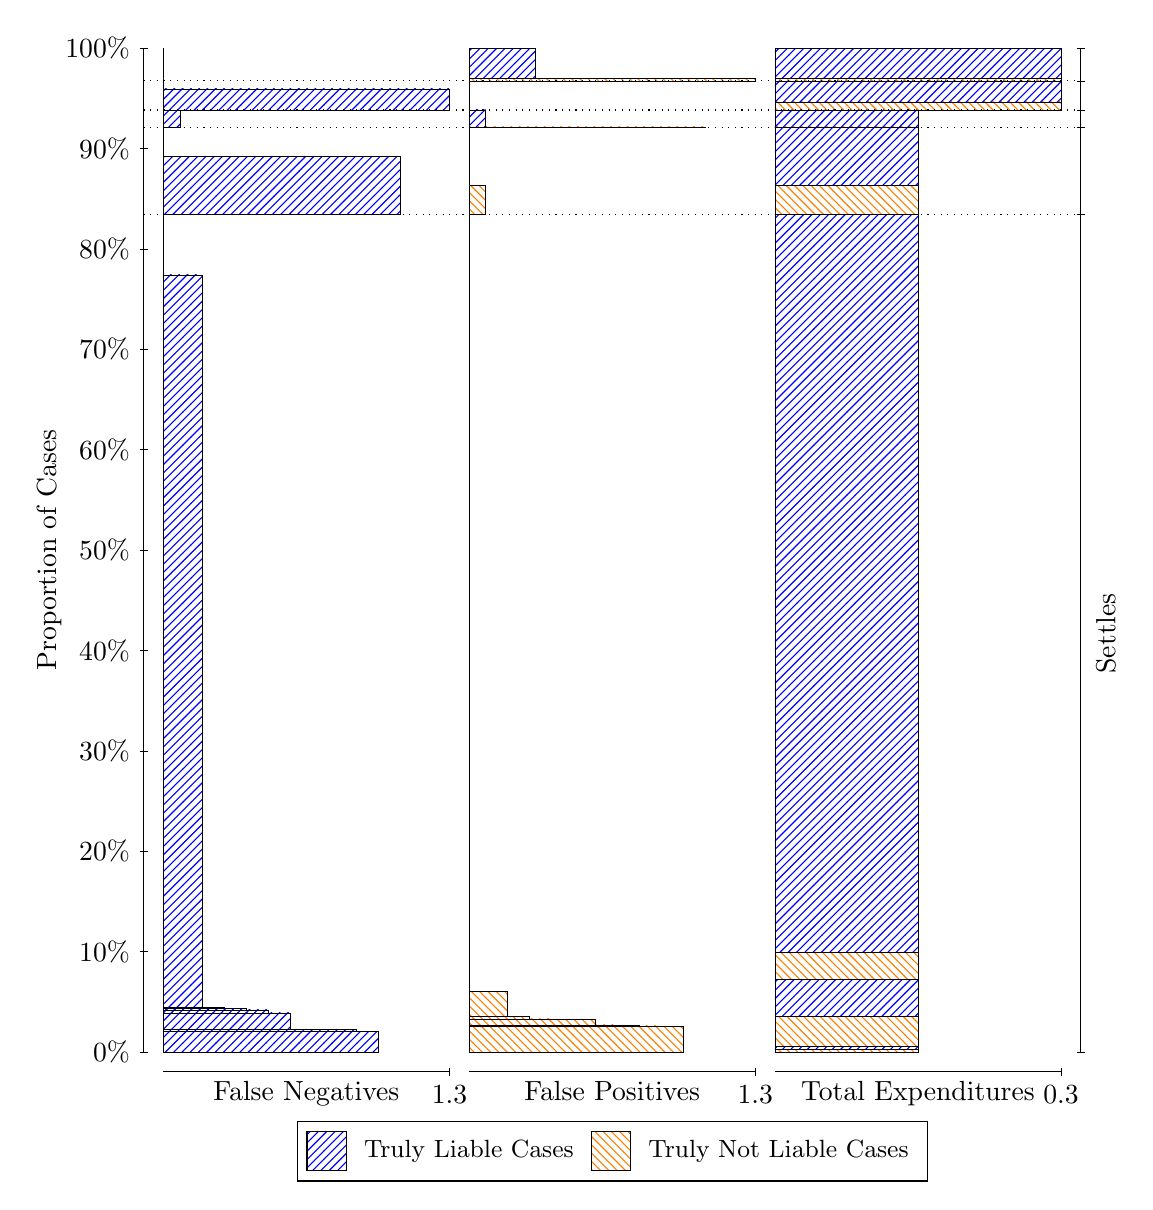
\begin{tikzpicture}
\draw[black, very thin] (1.5,1.75) -- (1.5,14.5);
\node[rotate=90, anchor=center] at (0.3, 8.125) {Proportion of Cases};
\draw[black, very thin] (1.45,1.75) -- (1.55,1.75);
\node[anchor=east] at (1.45, 1.75) {0\%};
\draw[black, very thin] (1.45,3.025) -- (1.55,3.025);
\node[anchor=east] at (1.45, 3.025) {10\%};
\draw[black, very thin] (1.45,4.3) -- (1.55,4.3);
\node[anchor=east] at (1.45, 4.3) {20\%};
\draw[black, very thin] (1.45,5.575) -- (1.55,5.575);
\node[anchor=east] at (1.45, 5.575) {30\%};
\draw[black, very thin] (1.45,6.85) -- (1.55,6.85);
\node[anchor=east] at (1.45, 6.85) {40\%};
\draw[black, very thin] (1.45,8.125) -- (1.55,8.125);
\node[anchor=east] at (1.45, 8.125) {50\%};
\draw[black, very thin] (1.45,9.4) -- (1.55,9.4);
\node[anchor=east] at (1.45, 9.4) {60\%};
\draw[black, very thin] (1.45,10.675) -- (1.55,10.675);
\node[anchor=east] at (1.45, 10.675) {70\%};
\draw[black, very thin] (1.45,11.95) -- (1.55,11.95);
\node[anchor=east] at (1.45, 11.95) {80\%};
\draw[black, very thin] (1.45,13.225) -- (1.55,13.225);
\node[anchor=east] at (1.45, 13.225) {90\%};
\draw[black, very thin] (1.45,14.5) -- (1.55,14.5);
\node[anchor=east] at (1.45, 14.5) {100\%};

\draw[black, very thin] (13.4,1.75) -- (13.4,14.5);
\draw[black, very thin] (13.35,1.75) -- (13.45,1.75);
\node[anchor=west] at (13.35, 1.75) {};
\draw[black, very thin] (13.35,12.383) -- (13.45,12.383);
\node[anchor=west] at (13.35, 12.383) {};
\draw[black, very thin] (13.35,13.494) -- (13.45,13.494);
\node[anchor=west] at (13.35, 13.494) {};
\draw[black, very thin] (13.35,13.713) -- (13.45,13.713);
\node[anchor=west] at (13.35, 13.713) {};
\draw[black, very thin] (13.35,14.084) -- (13.45,14.084);
\node[anchor=west] at (13.35, 14.084) {};
\draw[black, very thin] (13.35,14.5) -- (13.45,14.5);
\node[anchor=west] at (13.35, 14.5) {};

\draw[black, very thin, pattern color=blue, pattern=north east lines] (1.75,1.75) rectangle (4.475,2.0081);
\draw[black, very thin, pattern color=blue, pattern=north east lines] (1.75,2.0081) rectangle (4.1955,2.0345);
\draw[black, very thin, pattern color=blue, pattern=north east lines] (1.75,2.0345) rectangle (3.916,2.0393);
\draw[black, very thin, pattern color=blue, pattern=north east lines] (1.75,2.0393) rectangle (3.6365,2.0407);
\draw[black, very thin, pattern color=blue, pattern=north east lines] (1.75,2.0407) rectangle (3.3571,2.2478);
\draw[black, very thin, pattern color=blue, pattern=north east lines] (1.75,2.2478) rectangle (3.0776,2.2849);
\draw[black, very thin, pattern color=blue, pattern=north east lines] (1.75,2.2849) rectangle (2.7981,2.3006);
\draw[black, very thin, pattern color=blue, pattern=north east lines] (1.75,2.3006) rectangle (2.5186,2.3164);
\draw[black, very thin, pattern color=blue, pattern=north east lines] (1.75,2.3164) rectangle (2.2391,11.618);
\draw[black, very thin, pattern color=orange, pattern=north west lines] (1.75,11.618) rectangle (1.75,12.383);
\draw[black, very thin, pattern color=blue, pattern=north east lines] (1.75,12.383) rectangle (4.7545,13.122);
\draw[black, very thin, pattern color=orange, pattern=north west lines] (1.75,13.122) rectangle (1.75,13.494);
\draw[black, very thin, pattern color=blue, pattern=north east lines] (1.75,13.494) rectangle (1.9596,13.707);
\draw[black, very thin, pattern color=orange, pattern=north west lines] (1.75,13.707) rectangle (1.75,13.713);
\draw[black, very thin, pattern color=blue, pattern=north east lines] (1.75,13.713) rectangle (5.3833,13.981);
\draw[black, very thin, pattern color=orange, pattern=north west lines] (1.75,13.981) rectangle (1.75,14.084);
\draw[black, very thin, pattern color=orange, pattern=north west lines] (1.75,14.084) rectangle (1.75,14.113);
\draw[black, very thin, pattern color=blue, pattern=north east lines] (1.75,14.113) rectangle (1.75,14.5);
\draw[black, very thin, pattern color=orange, pattern=north west lines] (5.6333,1.75) rectangle (8.3583,2.0786);
\draw[black, very thin, pattern color=orange, pattern=north west lines] (5.6333,2.0786) rectangle (8.0788,2.0812);
\draw[black, very thin, pattern color=orange, pattern=north west lines] (5.6333,2.0812) rectangle (7.7994,2.0838);
\draw[black, very thin, pattern color=orange, pattern=north west lines] (5.6333,2.0838) rectangle (7.5199,2.0938);
\draw[black, very thin, pattern color=orange, pattern=north west lines] (5.6333,2.0938) rectangle (7.2404,2.1664);
\draw[black, very thin, pattern color=orange, pattern=north west lines] (5.6333,2.1664) rectangle (6.9609,2.1664);
\draw[black, very thin, pattern color=orange, pattern=north west lines] (5.6333,2.1664) rectangle (6.9609,2.1667);
\draw[black, very thin, pattern color=orange, pattern=north west lines] (5.6333,2.1667) rectangle (6.6814,2.1707);
\draw[black, very thin, pattern color=orange, pattern=north west lines] (5.6333,2.1707) rectangle (6.4019,2.2021);
\draw[black, very thin, pattern color=orange, pattern=north west lines] (5.6333,2.2021) rectangle (6.1224,2.5152);
\draw[black, very thin, pattern color=blue, pattern=north east lines] (5.6333,2.5152) rectangle (5.6333,12.383);
\draw[black, very thin, pattern color=orange, pattern=north west lines] (5.6333,12.383) rectangle (5.8429,12.755);
\draw[black, very thin, pattern color=blue, pattern=north east lines] (5.6333,12.755) rectangle (5.6333,13.494);
\draw[black, very thin, pattern color=orange, pattern=north west lines] (5.6333,13.494) rectangle (8.6378,13.499);
\draw[black, very thin, pattern color=blue, pattern=north east lines] (5.6333,13.499) rectangle (5.8429,13.713);
\draw[black, very thin, pattern color=orange, pattern=north west lines] (5.6333,13.713) rectangle (5.6333,13.816);
\draw[black, very thin, pattern color=blue, pattern=north east lines] (5.6333,13.816) rectangle (5.6333,14.084);
\draw[black, very thin, pattern color=orange, pattern=north west lines] (5.6333,14.084) rectangle (9.2667,14.113);
\draw[black, very thin, pattern color=blue, pattern=north east lines] (5.6333,14.113) rectangle (6.4718,14.5);
\draw[black, very thin, pattern color=orange, pattern=north west lines] (9.5167,1.75) rectangle (11.333,1.7857);
\draw[black, very thin, pattern color=blue, pattern=north east lines] (9.5167,1.7857) rectangle (11.333,1.8182);
\draw[black, very thin, pattern color=orange, pattern=north west lines] (9.5167,1.8182) rectangle (11.333,2.2039);
\draw[black, very thin, pattern color=blue, pattern=north east lines] (9.5167,2.2039) rectangle (11.333,2.6692);
\draw[black, very thin, pattern color=orange, pattern=north west lines] (9.5167,2.6692) rectangle (11.333,3.013);
\draw[black, very thin, pattern color=blue, pattern=north east lines] (9.5167,3.013) rectangle (11.333,12.383);
\draw[black, very thin, pattern color=orange, pattern=north west lines] (9.5167,12.383) rectangle (11.333,12.755);
\draw[black, very thin, pattern color=blue, pattern=north east lines] (9.5167,12.755) rectangle (11.333,13.494);
\draw[black, very thin, pattern color=orange, pattern=north west lines] (9.5167,13.494) rectangle (11.333,13.499);
\draw[black, very thin, pattern color=blue, pattern=north east lines] (9.5167,13.499) rectangle (11.333,13.713);
\draw[black, very thin, pattern color=orange, pattern=north west lines] (9.5167,13.713) rectangle (13.15,13.816);
\draw[black, very thin, pattern color=blue, pattern=north east lines] (9.5167,13.816) rectangle (13.15,14.084);
\draw[black, very thin, pattern color=orange, pattern=north west lines] (9.5167,14.084) rectangle (13.15,14.113);
\draw[black, very thin, pattern color=blue, pattern=north east lines] (9.5167,14.113) rectangle (13.15,14.5);
\draw[black, dotted] (1.5,12.383) -- (13.4,12.383);
\draw[black, dotted] (1.5,13.494) -- (13.4,13.494);
\draw[black, dotted] (1.5,13.713) -- (13.4,13.713);
\draw[black, dotted] (1.5,14.084) -- (13.4,14.084);
\draw[black, very thin] (1.75,1.5) -- (5.3833,1.5);
\node[anchor=north] at (3.5667, 1.5) {False Negatives};
\draw[black, very thin] (5.3833,1.45) -- (5.3833,1.55);
\node[anchor=north] at (5.3833, 1.45) {1.3};

\draw[black, very thin] (5.6333,1.5) -- (9.2667,1.5);
\node[anchor=north] at (7.45, 1.5) {False Positives};
\draw[black, very thin] (9.2667,1.45) -- (9.2667,1.55);
\node[anchor=north] at (9.2667, 1.45) {1.3};

\draw[black, very thin] (9.5167,1.5) -- (13.15,1.5);
\node[anchor=north] at (11.333, 1.5) {Total Expenditures};
\draw[black, very thin] (13.15,1.45) -- (13.15,1.55);
\node[anchor=north] at (13.15, 1.45) {0.3};

\node[black, centered, rotate=90] at (13.72, 7.0664) {Settles};





\draw (7.449999999999999,1.5) node[draw=none] (baseCoordinate) {};
\begin{scope}[align=center]
        \matrix[scale=0.5, draw=black, below=0.5cm of baseCoordinate, nodes={draw}, column sep=0.1cm]{
            \node[rectangle, draw, minimum width=0.5cm, minimum height=0.5cm, pattern=north east lines, pattern color=blue] {}; &
            \node[draw=none, font=\small] (B) {Truly Liable Cases}; &
            \node[rectangle, draw, minimum width=0.5cm, minimum height=0.5cm, pattern=north west lines, pattern color=orange] {}; &
            \node[draw=none, font=\small] (B) {Truly Not Liable Cases}; \\
            };
\end{scope}

\end{tikzpicture}
\end{document}